\documentclass[10pt,a4paper]{article}
\usepackage[utf8]{inputenc}
\usepackage{amsmath}
\usepackage{amsfonts}
\usepackage{amssymb}
\usepackage{graphicx}

\begin{document}




Na Figura~\ref{fig:matrix-similarity} é mostrado um exemplo de uma matriz de similaridade onde a intensidade do ponto($i,j$) representa a similaridade entre as sentenças $i$ e $j$. Observa-se que a matriz é simétrica, assim cada ponto na linha diagonal representa a similaridade quanto $i = j$ (ou seja, com a mesma sentença) e revela quadrados com maior concentração de pontos ao longo da diagonal. Essas regiões indicam porções de texto com maior coesão léxica.


  %--- Figura Visão Geral ---
  \begin{figure}[!h]
	  \centering
	  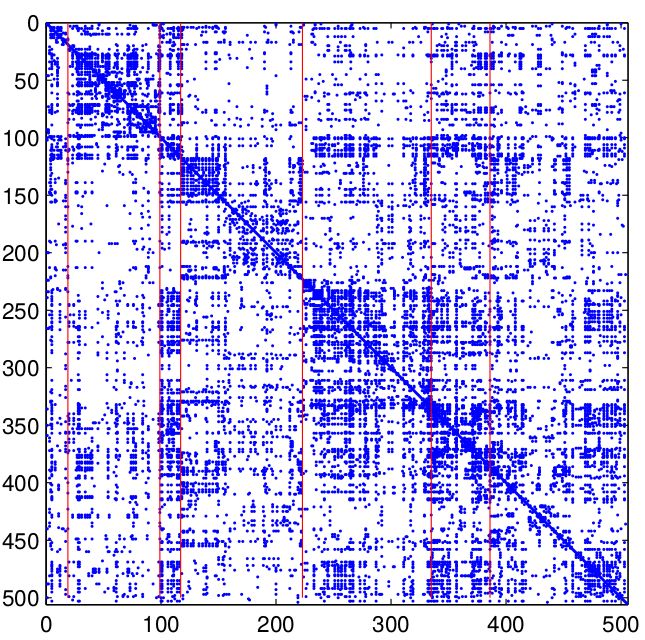
\includegraphics[width=1\textwidth]{c99.png}
	  \caption{\textit{DotPlot} da similaridade entre sentenças onde as linha verticais representam segmentos reais.}
	  \label{fig:matrix-similarity}
  \end{figure}



%%%%%%%%%%%%%%%%%%%%%%%
% - Falar do esquema de ranking;
% - Imagem com os passos e máscara 3x3;


% -? Após a contrução da matriz de ranking obtem-se um maior contraste entre facilitando a detecção de limites quando a queda de similaridade entre sentenças é mais sutil.


O processo de intentificação dos limites é baseado no método DotPloting~\cite{Reynar} que usa regiões com maior densidade em uma matriz de similaridades para determinar como os segmentos são distribuídos. Um segmento é definido por duas sentenças $i$ e $j$ que representam uma região quadrada ao longo da diagonal da matriz. 
%
%
%%%%%%%%%%%%%%
%
Seja $s_{i,j}$ a somatória dos \textit{rakings} de um segmento e $a_{i,j}$ sua área interior. Seja $B = \{b1,...,b_m\}$ a lista de $m$ segmentos.


Calcula-se a medida de densidade de uma região por 

\begin{equation}
D = 
\end{equation}


onde $s_k$  $a_k$ são a somatória dos valores dos rankings e a área de um segmento $k$ em $B$.

O processo incia com um único segmento formado por todas as sentenças do documento e o divide recursivamente em $m$ segmentos. Cada passo divide um dos segmentos em B no ponto $ij$ que maximiza D. O processo ser repte até que se atinja o número de segmento desejados ou um limiar de similaridade.
 



%%%%%%%%%%%%%%


\end{document}







%Assim, a matriz de similaridades é divida nas posições $i$ e $j$ que maximizam a função de densidade (Equação )

%O processo se repete até que se atinja o número desejado segmentos.



%Na Figura~\ref{fig:matrix-similarity} é mostrado um exemplo de uma matriz de similaridade onde a intensidade do ponto($i,j$) representa similaridade entre as sentenças $i$ e $j$ e cada ponto na linha diagonal representa a similaridade quanto $i = j$, ou seja, com a mesma sentença. Observa-se que a matriz é simétrica e revela quadrados ao longo da diagonal que indicam as regiões com maior coesão léxica.





%Na Figura~\ref{fig:matrix-similarity} é mostrado um exemplo de uma matriz de similaridade onde a intensidade do ponto($i,j$) representa similaridade entre as sentenças $i$ e $j$. Observa-se que a matriz é simétrica
%, assim cada ponto na linha diagonal representa a similaridade quanto $i = j$ (ou seja, com a mesma sentença) 
%e revela quadrados ao longo da diagonal que indicam as regiões com maior coesão léxica.


%representa a intensidade com que a i-ésima sentença é  similar a j-ésima sentença 

